\appendix
\clearpage
\section{Anhänge}
\subsection{Anwendungsfalldiagramm}
	\label{usecasefootersection}
\begin{figure}[!htb]
	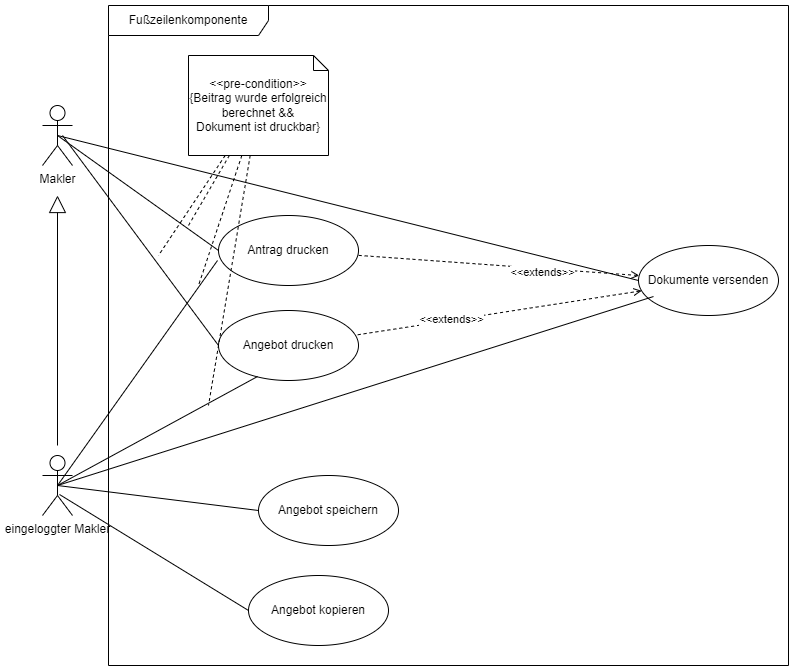
\includegraphics[width=\textwidth, height=\textheight, keepaspectratio]{anhang/usecase_footer.png}
	\caption{Anwendungsfalldiagramm der Fußzeilenkomponente}
	\label{usecasefooter}
\end{figure}

\subsection{Oberflächenabbildungen}
	\label{uisection}
\begin{figure}[!htb]
	
\includegraphics[width=\textwidth, height=\textheight, keepaspectratio]{anhang/mockup_footer.png}
	\caption{Mockup-Design der Fußzeile}
	\label{mockup}
\end{figure}
\begin{figure}[!htb]
	
\includegraphics[width=\textwidth, height=\textheight, keepaspectratio]{anhang/actual_footer.png}
	\caption{Tatsächliches Design der Fußzeile}
	\label{actualfooter}
\end{figure}
\begin{figure}[!htb]
	
\includegraphics[width=\textwidth,  keepaspectratio]{anhang/otr.png}
	\caption{Benutzeroberfläche OTR}
	\label{otr_figure}
\end{figure}